% Nallino, Part I p. 91: the horizon ABCD (centre E) with the lines AC and BD, the half DLB of the
% ecliptic above the horizon (an arc of a circle through B and D), the line from M through K, E and F to
% G, and the astrolabe at the lower left with its diameters TS and MK; the four quarters MERIDIES,
% ORIENS, OCCIDENS, SEPTENTRIONES. Circles, the arc and lines are least-squares fits to the printed ink;
% coordinates are PDF points of master page 180 less the origin (73.44, 279.06), y downward.
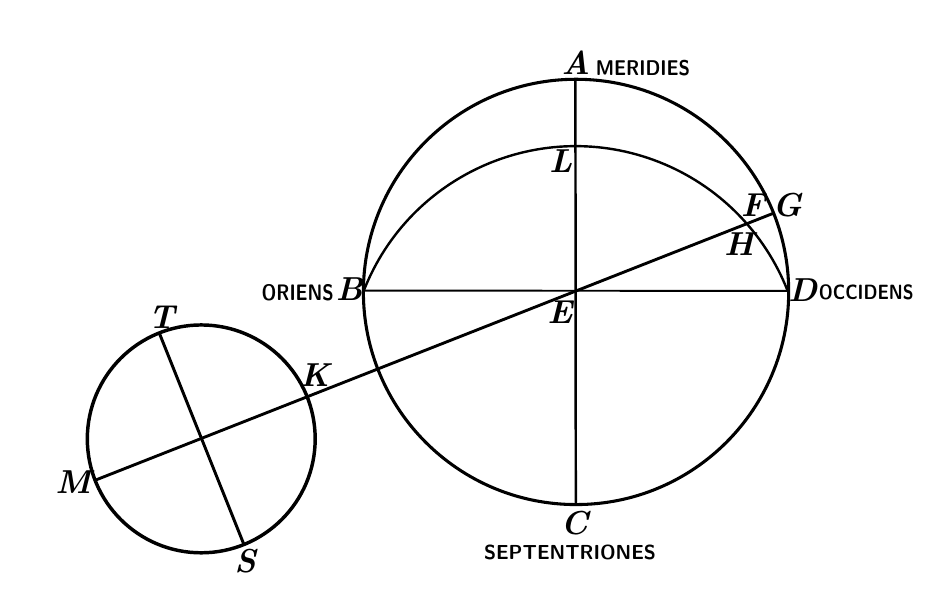
\begin{tikzpicture}[x=0.9915pt,y=-0.9915pt,line cap=butt,every node/.style={font=\fontsize{11.5}{11.5}\bfseries\itshape\selectfont,inner sep=0pt}]
\useasboundingbox (0,0) rectangle (325.00,200.00);
\draw[line width=1.11pt] (199.85,96.30) circle[radius=77.50];  % the horizon ABCD, centre E
\draw[line width=1.25pt] (63.26,149.86) circle[radius=41.52];  % the astrolabe, with its diameters TS and MK
\draw[line width=0.89pt] (199.62,18.80) -- (199.76,173.80);  % the line AC (south to north) through E
\draw[line width=0.71pt] (122.35,95.84) -- (277.35,95.91);  % the line BD (east to west) through E
\draw[line width=1.07pt] (47.96,111.27) -- (78.81,188.36);  % the diameter TS of the astrolabe
\draw[line width=1.04pt] (24.57,164.94) -- (271.84,67.61);  % the line from M through K, E and F to G (the side of the rule or the inside of the tube)
\draw[line width=0.87pt] (122.48,95.88) arc[start angle=201.40,end angle=338.72,radius=82.96];
\node at (199.76,12.99) {A};
\node at (194.31,48.79) {L};
\node at (264.36,64.59) {F};
\node at (276.86,64.59) {G};
\node at (259.21,78.74) {H};
\node at (117.27,95.46) {B};
\node at (282.43,95.55) {D};
\node at (193.99,103.66) {E};
\node at (48.77,105.36) {T};
\node at (104.61,126.57) {K};
\node at (16.61,165.77) {M};
\node at (79.24,194.27) {S};
\node at (199.19,180.55) {C};
\node at (224.25,14.60) {\normalfont\fontsize{8.5}{8.5}\sffamily\bfseries\selectfont \resizebox{34.00pt}{5.35pt}{MERIDIES}};
\node at (98.43,96.73) {\normalfont\fontsize{8.5}{8.5}\sffamily\bfseries\selectfont \resizebox{26.06pt}{5.62pt}{ORIENS}};
\node at (305.63,96.60) {\normalfont\fontsize{8.5}{8.5}\sffamily\bfseries\selectfont \resizebox{34.18pt}{5.18pt}{OCCIDENS}};
\node at (197.66,191.38) {\normalfont\fontsize{8.5}{8.5}\sffamily\bfseries\selectfont \resizebox{62.11pt}{5.09pt}{SEPTENTRIONES}};
\end{tikzpicture}
